\chapter{Feature Extraction}
\label{ch:FeatureExtraction}

Before diving into the novelty detection framework itself, the features to be used need to be defined and extracted from the data. Since our goal is to detect a novel behaviour, we are interested in both \quoted{time-domain} and \quoted{frequency-domain} features. The former are used to capture the temporal evolution of the signal, while the latter are used to capture the spectral content of the signal. In this chapter, we will first introduce the reference dataset that will be used to test the framework and then we will describe the features that will be used in the framework.

\section{Reference dataset}
In the field of \gls{nd}, a famous bearing vibration dataset has been collected from the Center for Intelligent Maintenance Systems (\gls{ims}) of the University of Cincinnati and made available online on the \gls{nasa} website \cite{lee2007bearingdataset}. 
Let's take this as a starting point for our work. The dataset contains the vibration measurements collected at a sampling frequency $f_s=20\si{\kHz}$ of four forced-lubricated bearings. The shaft was kept constant at $2000$rpm during the data collection. The test rig is shown in \autoref{fig:IMS_bearing_dataset} and the test parameters are summarized in \autoref{tab:IMS_test_parameters}, that also shows the type of faults that happened in each repetiotion of the test.

\begin{figure}
    \centering
    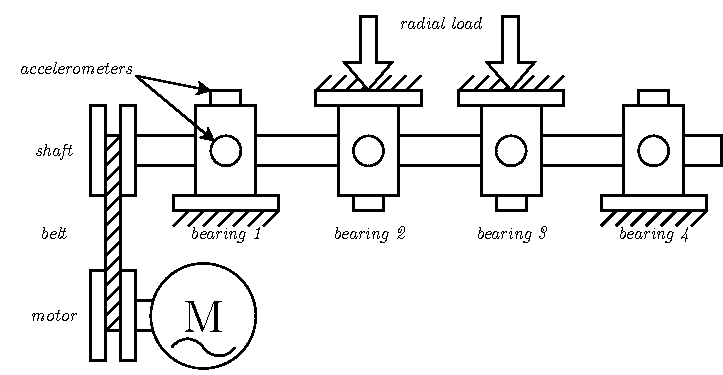
\includegraphics[scale=1]{images/FeatureExtraction/testrig.pdf}
    \caption{The test rig used by \cite{lee2007bearingdataset}}
    \label{fig:IMS_bearing_dataset}
\end{figure}

% \usepackage{tabularray}
\begin{table}
    \centering
    \caption{Test setup provided by \cite{lee2007bearingdataset}}
    \label{tab:IMS_test_parameters}
    \resizebox{\linewidth}{!}{%
    \begin{tblr}{
      cell{2}{1} = {t},
      cell{2}{2} = {t},
      cell{3}{1} = {t},
      cell{3}{2} = {t},
      cell{5}{1} = {t},
      cell{5}{2} = {t},
      cell{6}{1} = {t},
      cell{6}{2} = {t},
      cell{7}{1} = {t},
      cell{7}{2} = {t},
      hline{1,8} = {-}{0.08em},
      hline{2} = {-}{},
    }
     & \textbf{Set No. 1} & \textbf{Set No. 2} & \textbf{Set No. 3}\\
    \textbf{Recording Duration} & 22/10/2003 - 25/11/2003 & 12/02/2004 - 19/02/2004 & 04/03/2004 - 04/04/2004\\
    \textbf{No. of Files} & 2156 & 984 & 4448\\
    \textbf{No. of Channels} & 8 & 4 & 4\\
    \textbf{Channel Arrangement} & {Bearing 1 ch 1  2\\Bearing 2 ch 3  4
    \\Bearing 3 ch 5  6
    \\Bearing 4 ch 7 \& 8~ ~~} & {Bearing 1 ch 1\\Bearing 2 ch 2\\Bearing 3 ch 3\\Bearing 4 ch 4 ~} & {Bearing 1 ch 1\\Bearing 2 ch 2\\Bearing 3 ch 3\\Bearing 4 ch 4~ ~~}\\
    \textbf{File Recording Interval} & 5 or 10 min & 10 min & 10 min\\
    \textbf{Fault type } & {Bearing 3: inner race defect\\Bearing 4: roller element defect} & Bearing 1: outer race failure & Bearing 3: outer race failure
    \end{tblr}
    }
    \end{table}

\section{Time-domain features}
